{\color{gray}\hrule}
\section{Cross Bones Eyes (349,564) and (359,564)}
{\color{gray}\hrule}

\subsection{10 Pixels Apart?}

The next two most contested pixels are exactly 10 pixels apart in the x axis. Due to their close proximity, I hypothesized these two pixels correlated with the same art piece. So, I viewed the pixels placed around them to determine their correlation. From figure 3, it is clear that both pixels correlated to the eyes of the skeleton. 

\begin{figure}[H]
\centering
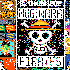
\includegraphics{visuals/349_564_35_80_mode_1}
    \caption{Most recent pixel placements in a 70x70 grid around centering on (349, 564) }
\end{figure}

\subsection{Why The Eyes?}

Despite encompassing an area roughly 35 x 65 pixels, the eyes drew the most user placements. From this, I assumed that it may have been a conflict between two groups that wanted different eye colors for the skeleton. To verify this assumption, I looked into to the top colors used at the locations. If a conflict occurred, then the two top colors should be the same for both eyes and should be relatively much larger than the other colors. 
 The right eye had 34726 black pixels placed, 26940 light blue pixels, and 1656 red pixels as the top three. The left eye had 27804 black pixels placed, 19404 light blue pixels, and 2120 red pixels as the top three. From this, it can be seen that black and light blue were orders of magnitude greater than the next most common color and that it was likely the product of the conflict between two groups.

\begin{figure}[H]
\centering
\animategraphics[loop,autoplay, width=100pt]{3}{visuals/349_564_10_mode_0_}{0}{83}
    \caption{Animation of most common placements around the left eye. \\ Note: The center of the eyes remain black during the animation as it was most fiercely defended, but this can be seen at other parts of the eyes as users were more lax around these parts}
\end{figure}


\subsection{Why Black And Blue?}
The original art piece is One Piece's Crossbones maintained by r/onepiece and the other group is from r/Undertale. The r/Undertale community attempted to convert every skeleton into Sans with blue eyes and they focused on Crossbones. The fierce defense and attempt to convert Crossbones drove user activity specifically at the eyes.